Full page circuit diagrams of CPU sub-systems as described in \ref{CPUDes}.
\begin{figure*}
    \centering
    \includegraphics[width=0.9\textheight, angle=90]{Images/ALU.pdf}
    \caption{Circuit diagram of the arithmetic logic unit}
    \label{fig:enter-label}
\end{figure*}

\clearpage
\begin{figure*}
    \centering
    \includegraphics[width=\textheight, angle=90]{Images/InstructionRegister.pdf}
    \caption{Circuit diagram of the Instruction Register}
    \label{fig:enter-label}
\end{figure*}

\clearpage
\begin{figure}
    \centering
    
\includegraphics[width=\textheight, angle=90]{Images/Step Counter.pdf}
    \caption{Circuit diagram of the Step Counter}
    \label{fig:enter-label}
\end{figure}


\begin{figure}
    \centering
    \includegraphics[width=\textheight, angle=90]{Images/ProgramCounter.pdf}
    \caption{Circuit diagram of the Program Counter}
    \label{fig:enter-label}
\end{figure}

\clearpage
\begin{figure*}
    \centering
    \includegraphics[width=\textheight, angle=90]{Images/Stack.pdf}
    \caption{Circuit diagram of the Stack}
    \label{fig:enter-label}
\end{figure*}

\clearpage
\begin{figure*}
    \centering
    \includegraphics[height=\textheight]{Images/ScratchPad.pdf}
    \caption{Circuit diagram of the Scratch Pad}
    \label{fig:enter-label}
\end{figure*}

\clearpage
\begin{figure*}
    \centering
    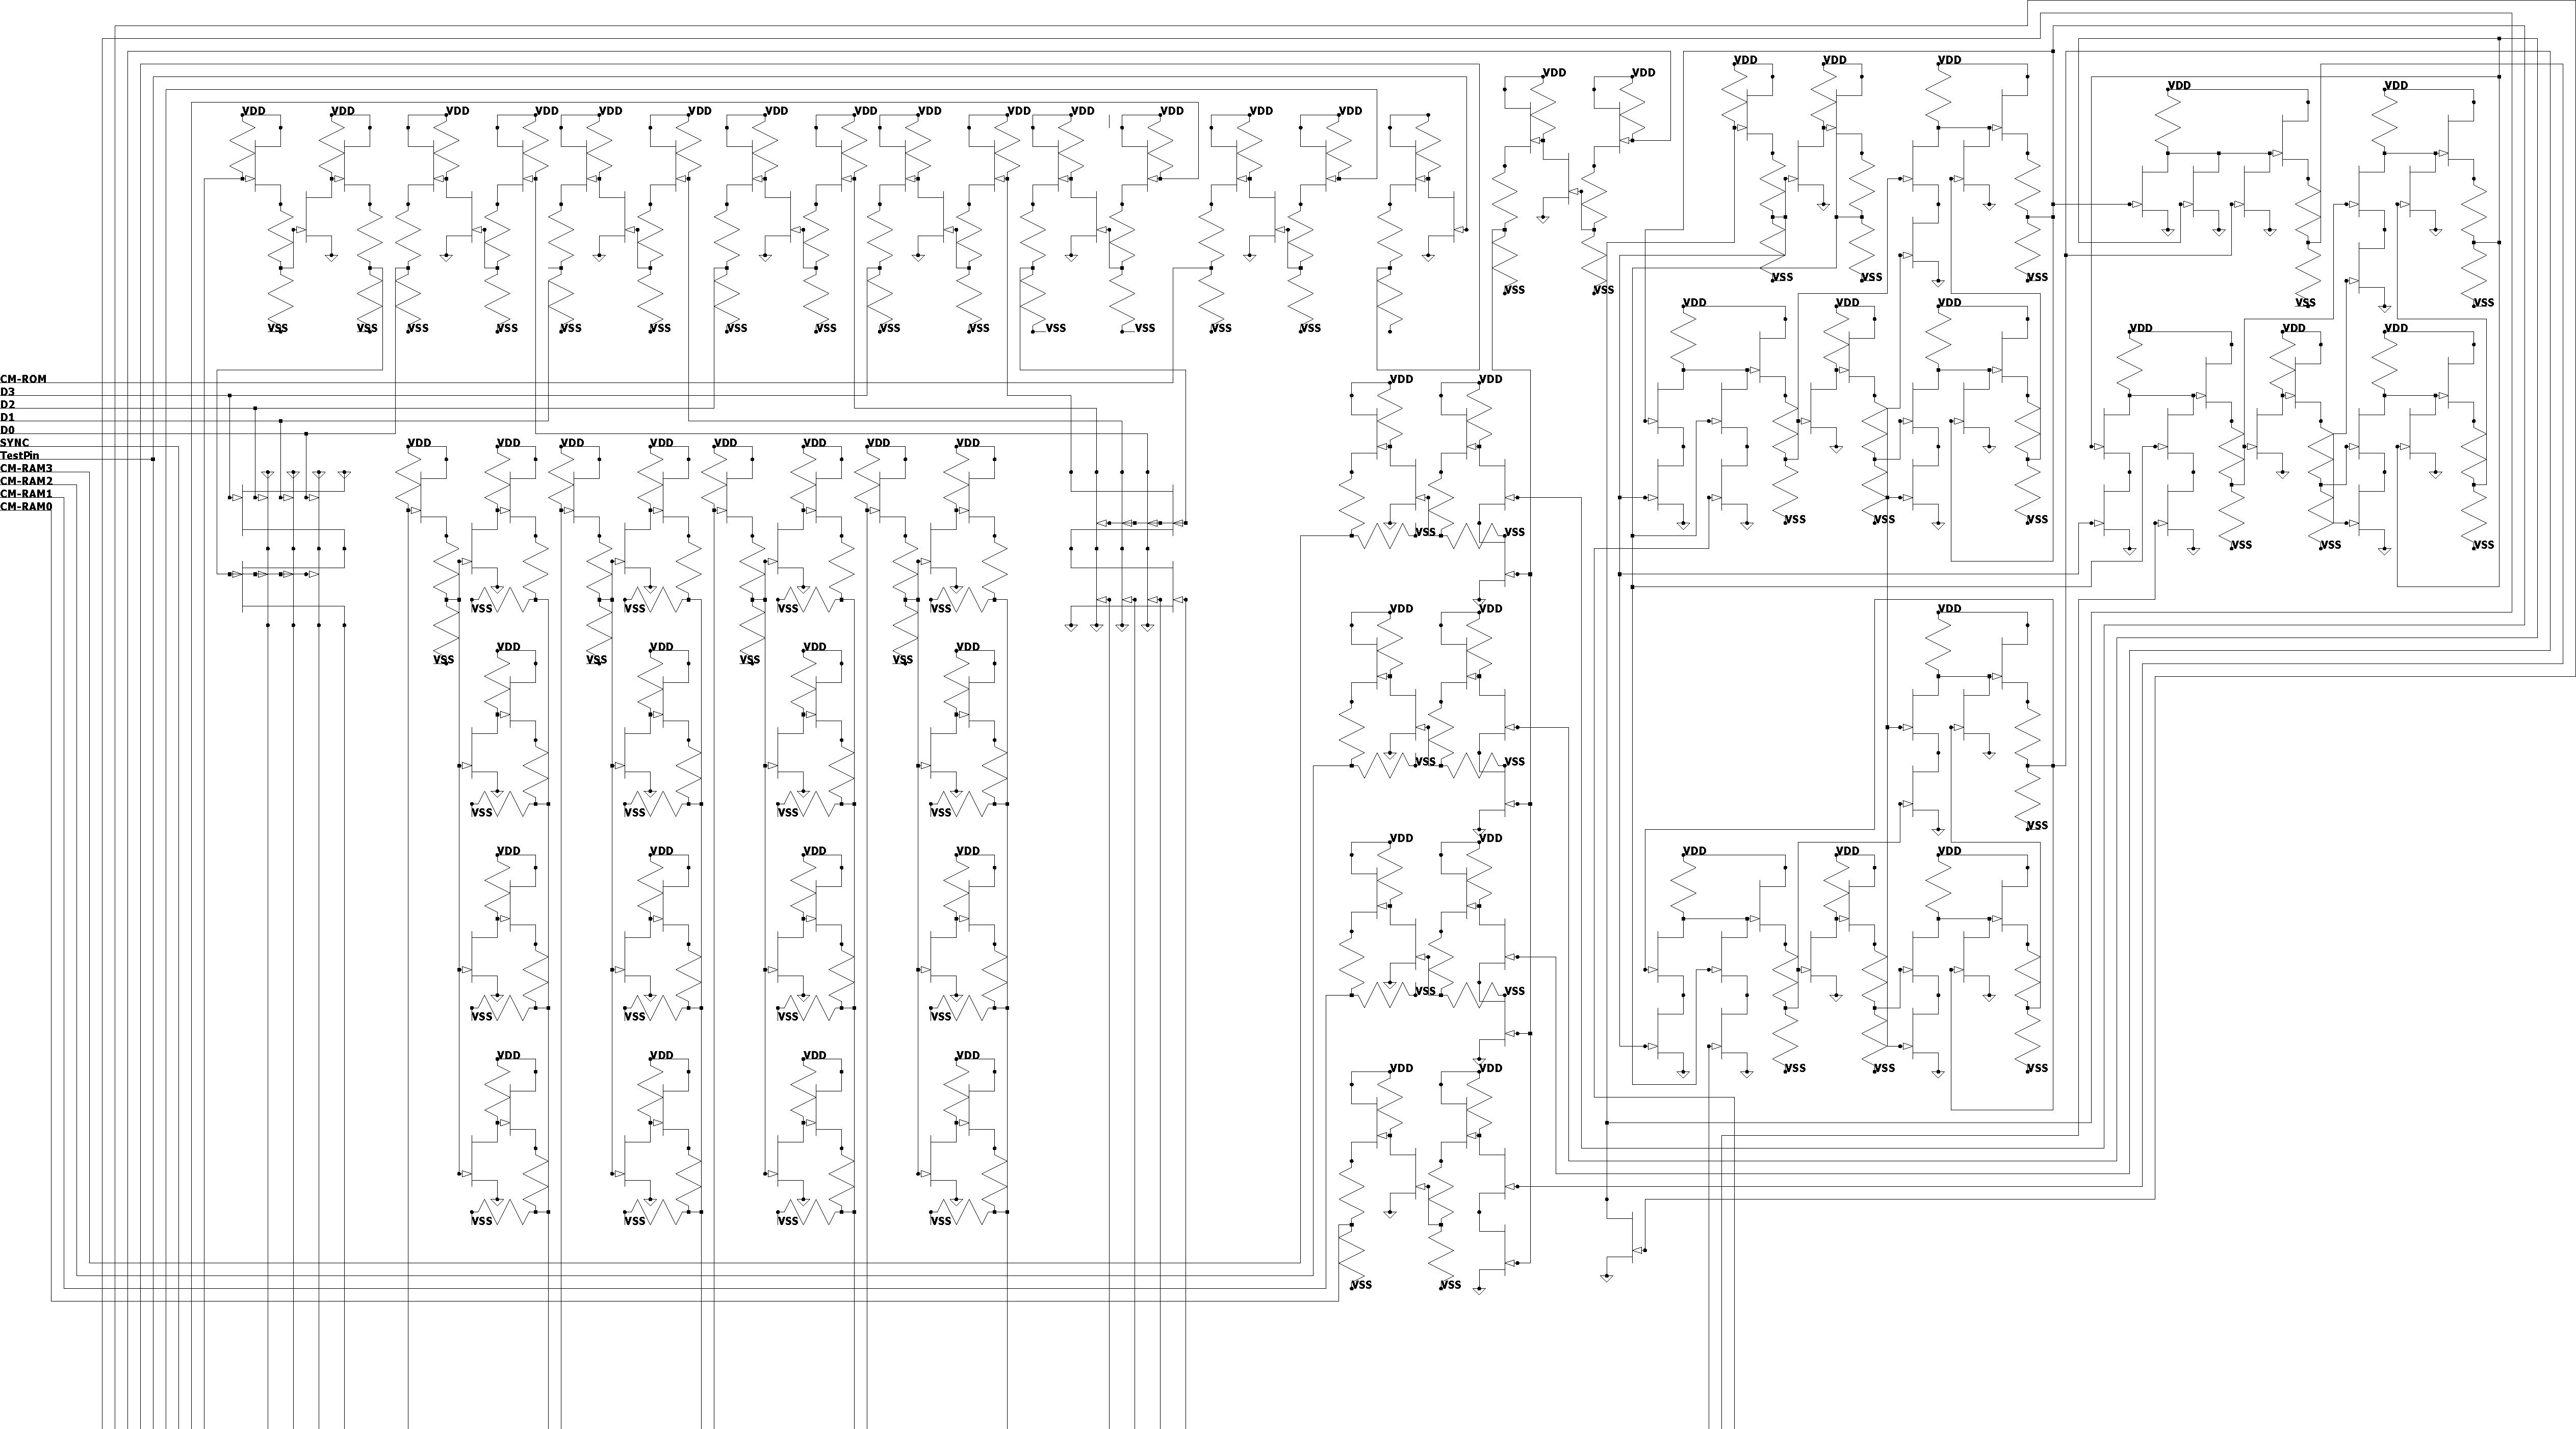
\includegraphics[width=\textheight, angle=90]{Images/Pins.pdf}
    \caption{Circuit diagram of the Pins}
    \label{fig:enter-label}
\end{figure*}

\clearpage
\begin{figure*}
    \centering
    \includegraphics[width=\textheight, angle=90]{Appendices/ROMUnannotated.pdf}
    \caption{Circuit diagram of the computational part of the ROM}
    \label{fig:enter-label}
\end{figure*}